\documentclass[output=paper]{langsci/langscibook}
\ChapterDOI{10.5281/zenodo.573787}



\title{Dependency and relative determination in language acquisition: The case of {Ku Waru}}
\shorttitlerunninghead{Dependency and relative determination in children’s language acquisition}

\author{Alan Rumsey\affiliation{Australian National University}
}
%\abstract{In this chapter I discuss what I take to be examples of dependency in children’s learning of Ku Waru, a Papuan language spoken in the Western Highlands Province of Papua New Guinea\footnote{For further details concerning the Ku Waru language and its social setting see \citet{Merlan1991}. }. The first example is a phonological one and has to do with the order of children’s acquisition of the four Ku Waru lateral consonant phonemes. The other example is syntactic and has to do with the order of acquisition of simple verbs and two kinds of phrasal verb construction: adjunct+verb constructions and serial verb constructions. I argue that both of these examples show dependencies based on two kinds of constraining factors: 1) intrinsic simplicity \textit{vs} complexity along dimensions which are common to all languages; 2) relational, language specific forms simplicity \textit{vs} complexity which have to with degrees of ‘pattern congruity’ or ‘structural congruence’ within phonological and syntactic systems respectively.}

\begin{document}
\maketitle

\il{Papuan} \is{phonology} \is{syntax} \is{phrasal verb constructions} \is{serial verb constructions}
\noindent In this chapter I discuss what I take to be examples of dependency in children’s learning of \ili{Ku Waru}, a \ili{Papuan} language spoken in the Western Highlands Prov\-ince of Papua New Guinea.\footnote{For further details concerning the \ili{Ku Waru} language and its social setting see \citet{Merlan1991}.} The first example is a phonological one and has to do with the order of children’s acquisition of the four \ili{Ku Waru} lateral consonant phonemes. The other example is syntactic and has to do with the order of acquisition of simple verbs and two kinds of phrasal verb construction: adjunct+verb constructions and serial verb constructions. I argue that both of these examples show dependencies based on two kinds of constraining factors: 1) intrinsic simplicity \textit{vs} complexity along dimensions which are common to all languages; 2) relational, language specific forms of simplicity \textit{vs} complexity which have to with degrees of ``pattern congruity" or ``structural congruence" within phonological and syntactic systems respectively. \is{simplicity vs. complexity} \is{pattern congruity} \is{structural congruity}

\section{\ili{Ku Waru} laterals and their acquisition}

\ili{Ku Waru} belongs to the \ili{Trans-New Guinea} family of \ili{Papuan} Languages \citep{Pawley2009}. The \ili{Ku Waru} phonemic inventory is shown in Tables \ref{tab:rumsey:1} and \ref{tab:rumsey:1vowels}.  The characters shown in parentheses are the ones in the practical orthography that is used in \sectref{sec:rumsey:2}.

\begin{table}
\caption{\ili{Ku Waru} phonemic inventory: Consonants}
\label{tab:rumsey:1}                                 

\begin{tabularx}{\textwidth}{lXXXXX}
\lsptoprule
& Labial & Apico-Alveolar & Palatal & Velar\\
\midrule
Plain stop & p & t &  & k\\
Fricative &  & s &  & \\
Prenasalized stop & mb (b) & nd (d) & ɲd͡ʒ (j) & ŋg (g)\\
Nasal & m & n & ɲ (ny, yn) & ŋ (ng)\\
Continuant & w & r & j (y) & \\
\\
% \lspbottomrule
\end{tabularx}

\medskip

\begin{tabularx}{\textwidth}{lXXXX} 
% \lsptoprule
& Retroflex \newline flap & Alveolar continuant & Palatal \mbox{continuant} & Prestopped \mbox{velar}\\
\midrule
Lateral & {ɺ̢  (rlt)} & l (\textit{l}\,) & {ʎ} (ly, yl) & {{\gL} (l)}\\
\lspbottomrule
\end{tabularx}

\end{table}

\begin{table}
\caption{\ili{Ku Waru} phonemic inventory: Vowels}
\label{tab:rumsey:1vowels}                                 

\begin{tabular}{llcrr}
% \lsptoprule
& Front &  & Back & \\
\midrule
High & i &  & u & \\
Mid & ~~~e &  & o~~~ & \\
Low &  & a &  & \\
% \lspbottomrule
\end{tabular}
\end{table}

The phonemes in \tabref{tab:rumsey:1} that I focus on in this chapter are the laterals. All four of them can occur word initially, medially and finally. Below are some examples, which include a minimal quadruplet in medial position (koɺa / ko{ʎ}a / ko{\gL}a / kola) and near-minimal contrasting forms in other positions.
 
\vspace{5mm}
\noindent
\textbf{Retrofex lateral flap}  /ɺ̢/.
\ea
\ea
/ɺim/           →   [ɺ̢im] a woman’s name
\ex
/(kera) koɺa/   → [(k{ɛ}r{ʌ}) koɺ̢{ʌ}] ‘(bird) chicken’
\ex
/(kum) piniɺ/  → [(kum)pinIɺ̢] ‘(ear) eardrum’
\z
\z

\noindent
\textbf{Palatal lateral continuent} /ʎ/. In word-initial and word-medial position this consonant is voiced and in word-final position it is voiceless. Examples are: 

\ea
\ea
/{ʎ}api/        →  [{ʎ}api] ‘fog’
\ex
/ko{ʎ}a/       →  [ko{ʎ}{ʌ}] ‘place’
\ex
/pa{ʎ}/       →  [pa{ʎ̥}]  ‘all’
\ex
/kundu{ʎ}/  →  [kundu{ʎ̥}] ‘red’
\z
\z

\noindent
\textbf{Prestopped velar lateral} /{\gL}/. This is a complex phoneme which in effect combines a velar stop and a velar lateral approximant. When producing it the back of the tongue is first bunched and placed against the velum as for the onset of a velar stop, but instead air is then released to both sides over the bunched tongue. In initial and medial position this phoneme is voiced, and in final position it is voiceless. Examples are:
\ea
\ea
/{\gL}apa/    →  [{\gL}ap{ʌ}] ‘father’
\ex
/ko{\gL}a/   →  [ko{\gL}{ʌ}] ‘cry’
\ex
/pa{\gL}a/    →  [pa{\gL}{ʌ}]  ‘fence post’
\ex
/wa{\gL}/    →  [wa{\kL}]  ‘string bag’
\ex
/pu{\gL}/    →  [pu{\kL}]   ‘base’
\z
\z

Although phonetically complex, this phoneme is by no means a marginal one in \ili{Ku Waru}. It is in fact the most frequently occurring lateral in the language. Given that it involves both velar occlusion and lateral approximation it is not inevitable that this phoneme should be classed as a lateral rather than a stop. I agree with \citet{François2010} that the choice in such cases is best made on language-internal, distributional grounds rather than purely phonetic ones, and will pre\-sent evidence of that kind below.
\vspace{5mm}

 \noindent
\textbf{Apico-alveolar /l/.} This sound has come into the phonemic inventory of \ili{Ku Waru} only since the arrival into the region of the mainly \ili{English}-based lingua franca \ili{Tok Pisin}, which happened in the 1930s. This is evident from the fact it occurs only in loan words from that language. 

Examples are:

\ea
\ea
\textit{lo} ([lo]), ‘law’, from Tok  Pisin \textit{lo} ‘law’, 
\ex
\textit{kela} ([k{ɛ}la]), from \ili{Tok Pisin} \textit{kela} ‘bald head’
\ex
\textit{kola} ([kol{ʌ}] from \ili{Tok Pisin} \textit{kola} ‘cola, soft drink’
\ex
\textit{gol} ([gol]), from \ili{Tok Pisin} \textit{gol} ‘gold’  
\z
\z

The adoption into \ili{Ku Waru} of /l/ as a phoneme (albeit still a marginal one) was probably facilitated by two preexisting patterns.

The first is that, although /l/ had not been present as a phoneme, [L] and [l] had already been present, as allophones of /{\gL}/ before stop consonants. Examples are:


\renewcommand{\eachwordone}{\upshape}
\ea
\gll 
/mo{\gL}-ku-r/                → [moLkur].\\
{be/stay-}{\textsc{ppr-1sg}}\\
\glt   ‘I am (staying)'
\z

\ea
\gll /sumbu{\gL}(u) tu$\lambda$/        → [sumbultuʎ̥] \\
darkness hit:\textsc{ppl}\\
\glt ‘night’
\z

\ea
/{\gL}ku/                        → [Lku]  \\
‘house’
\z


\renewcommand{\eachwordone}{\itshape}

The appearance of lateral continuants as allophones of /{\gL}/ when it occurs in consonant clusters provides evidence for grouping /{\gL}/ with the laterals rather than stops with respect to its manner of articulation. That interpretation is further supported by the fact that the velar positions in the two stop series are already filled by /k/ and /g/, which are invariably pronounced as stops, whereas /{\gL}/ loses its stop quality in this environment but retains its lateral quality as it does in all other environments. 

\is{baby talk register} The second pre-existing pattern that may have facilitated the adoption of /l/ from \ili{Tok Pisin} into \ili{Ku Waru} as a phoneme is that [l] has long been present as a pronunciation of /{\gL}/ in the baby talk register of \ili{Ku Waru}. It is used not only by children, between the ages of approximately 20 months and three years, but also by adults and older children when speaking to them. Examples are shown in Table \ref{tab:rumsey:2}.

\begin{table}
\begin{tabular}{lll}
\lsptoprule
\textbf{Adult form} & \textbf{Baby talk form} & \textbf{Meaning}\\
\midrule
o{\gL}a & ola & up\\
maɲa mo{\gL}a & mana mola & Sit down!\\
mo{\gL} ({\textgreater}[mo{\kL}]) & mol & no\\
\lspbottomrule
\end{tabular}
\caption{Some \ili{Ku Waru} baby talk forms}
\label{tab:rumsey:2}
\end{table}

Most children do not learn to produce adult-like versions of the {\gL}/{\kL} sound until they are 5-6 years old. In the meantime, as alternative pronunciations of it they use not only [l] as shown above, but also [k], [g], and later [ɣ] and [x]. Interestingly, adults and older children when speaking to children never use those sounds as baby talk realizations of /{\gL}/, only [l].

The facts that I have reviewed above regarding \ili{Ku Waru} laterals can, I believe, be at least partially accounted for in terms of relative determination, that is of tendencies that are widely attested in the world’s languages and affect how children learn them. The first thing to note in this respect is that from a comparative-typological\is{comparative typology}\is{typology} perspective the \ili{Ku Waru} inventory of laterals as described above is very unusual. In a survey of 567 of the world’s languages, \citet{MaddiesonLateralConsonants2013} found that by far the most common lateral was /l/, which was found in 76.7\% of the languages (cf. \citealt[153--154]{Ladefoged2001}; \citealt{Ladefoged1977}; \citealt{Ladefoged1996}). Only 9.5\% of the languages in \citegen{MaddiesonLateralConsonants2013} sample had lateral obstruents. The inventory of \ili{Ku Waru} laterals before the adoption of /l/ from \ili{Tok Pisin} was even more unusual: only 8 or 1.4\% of the languages had lateral obstruents but not /l/ (ibid). Of those 8 languages only 5 had two or more obstruent laterals (Maddieson, personal communication March 2016), which places \ili{Ku Waru} in a class that includes only 0.9\% of the sample. 

But here I would argue that the exception proves the rule – the rule of what I have called ``relative determination". This is true at two different levels – that of distributional patterns within the language and that of speakers’ metalinguistic awareness of degrees of complexity \textit{vs} simplicity. With respect to the first level, as I have shown above, even before the adoption of /l/ into \ili{Ku Waru} from \ili{Tok Pisin}, [l] and [L] were already present in \ili{Ku Waru} within a particular environment, namely, when preceding a stop.  I would take this to be an instance of the ubiquitous tendency that \citet{DeLacyMarkedness2006} demonstrates in detail and describes in the following terms: ``if there is synchronic non-assimilative, non-dissimilative neutralization $\beta$ \textbf{→} $\alpha$ in some prosodic environment, there is a markedness hierarchy \is{markedness!hierarchies} in which a feature value of $\beta$ is more marked than a related feature value of $\alpha$" (73)\footnote{Three aspects of this formulation call for comment in the present context. First, while the loss of the velar-stop component of /{\gL}/ before k might be thought of as a dissimilation from the following velar stop, this is counter-indicated by the fact that the same thing happens before t. Second, de Lacy’s use of the term ‘neutralization’ might be thought to render his generalization inapplicable in this case because the process in question does not involve a loss of phonemic contrast between /{\gL}/ and any other phoneme. But de Lacy’s use of the term neutralization does not entail loss of contrast \citep[110]{DeLacyMarkedness2006}. Third, lest De Lacy’s formulation appear tautological one must bear in mind that the markedness hierarchies he refers to are not ad hoc ones inferred from single cases but are intended to be universal and are constantly being tested against data from the world’s languages and refined on that basis.}. Here, where the $\beta $ term is /{\gL}/ and the $\alpha$ term is [L], the relevant feature is pre-occlusion, which disappears, leaving only the lateral continuant with which it is otherwise co-articulated. De Lacy’s generalization – which is consistent with the results of decades of work on markedness – definitely holds up in this case and is further supported by it, since consonants that involve coarticulation have ever since the foundational work of Trubetzkoy (\citeyear{Trubetskoy1931}, \citeyear{Trubetskoy1969}[1939]; cf. \citealt[42]{Baltaxe1978}) been regarded as more highly marked in their manner of articulation than those that do not.

\is{baby talk register} At the other level, that of metalinguistic awareness, it is surely no accident that the variant of /{\gL}/ that adults have settled upon as its baby talk equivalent is precisely the one that Maddieson has shown to be by far the most common one around the world: [l]. No doubt that has been determined in part by the fact that [l] is the first lateral sound that \ili{Ku Waru} children are able to produce. But it also seems to have been determined in part by the language-specific phonological status of /{\gL}/ within \ili{Ku Waru} as a lateral rather than as a stop.\footnote{In his very valuable comparative discussion of languages with velar laterals, \citet{François2010} convincingly demonstrates that {\gL} sounds are fundamentally ambiguous with respect their manner-of-articulation status as between (laterally released) stop and (pre-stopped) lateral. Based on his work on \ili{Hiw}, the only \ili{Austronesian} language known to have a {\gL} sound (which he analyses convincingly as a lateral phoneme) and with a speaker of the \ili{Papuan} language \ili{Ekari}, François was able to confirm that \ili{Ekari} has ‘exactly the same sound’, which is however, best regarded phonologically as a stop, for distributional and phonotactic reasons presented in \citet{Doble1987}. François reports that the same is true of \ili{Laghuu}, a \ili{Tibeto-Burman} language as described by \citet{Edmondson1999}.}

\section{The acquisition of \ili{Ku Waru} verbs, verb complexes and copular clauses}\label{sec:rumsey:2}
\subsection{Verbs, verb complexes and copular clauses in \ili{Ku Waru} adult speech}

\ili{Ku Waru} is typical of \ili{Trans-New Guinea} languages in having strictly verb-final syntax and three different kinds of finite verbs / verbal constructions as follows:

\begin{enumerate}
\item  \textsc{Simple verbs,} consisting of a root and suffixes specifying person/number and tense/aspect/mode. Examples are:

\ea
\ea
\gll   kang-ayl      \textbf{pu-ku-m}   \\
            boy-\textsc{def}      go-\textsc{ppr}-\textsc{3sg}     \\
\glt            `The boy is going.'                   
\ex
\gll kang-ayl-n       tauwu-ti      \textbf{nu-ru-m}\\
       boy-\textsc{def}-\textsc{erg}    banana-\textsc{idf}  eat-\textsc{rp}-\textsc{3sg}\\
\glt  `The boy ate a banana (before yesterday).'
\z
\z

\is{phrasal verb constructions} \item  \textsc{Adjunct+verb constructions (AVC)} consisting of an inflecting verb root immediately preceded by another word which functions as a  ``verbal adjunct".\footnote{For an introductory comparative discussion of these constructions in \ili{Papuan} languages see \citet[117--123]{Foley1986}. For further discussion of the AVC in \ili{Ku Waru} see \citet{MerlanForthcoming}.} Examples are: 

\ea
  \ea
  \gll kang-ayl      \textbf{nok}      \textbf{to}-\textbf{ku-m}     \\
      boy-\textsc{def}      cough    hit-\textsc{ppr}-\textsc{3sg}            \\
\glt	      `The boy is coughing.'
  \ex
      \gll na-n    no      \textbf{odi}   \textbf{le-bu}\\
	I-\textsc{erg}  water  pour    put.in.place-\textsc{fut}:\textsc{1sg}\\
  \glt `I will pour water.'
  \z
\z

All of the inflecting verbs that are used in these constructions can also be used without an adjunct, in which case their meanings are lexically more specific than when used with them. This can be seen in (9a) and (9b), where the verbs have been glossed with the meanings that they have when used without adjuncts. 

\is{serial verb constructions} \item \textsc{Serial verb constructions (SVC)}, comprising a sequence of two or more verbs, the final one inflected like a simple verb as in (8) and the preceding one(s) inflected with a ``non-final" suffix showing person and number but not tense, aspect or mode. Examples are:

\ea
\ea   
\gll na     langi    mare      \textbf{me-b}        \textbf{o-ku-r.}\\
        I        food     some      carry-\textsc{nf}:1    come-\textsc{ppr}-\textsc{1sg}\\
       \glt `I am bringing some food.'
\ex
\gll kewa-n       koi-d       teman-ti   \textbf{kodu-pa}       \textbf{nyi-m}\\
        kewa-\textsc{erg}  koy-\textsc{dat}  story-\textsc{idf}  pull-\textsc{nf}:\textsc{3sg}    say-\textsc{prf}:\textsc{3sg}\\
\glt        `Kewa told a story to \ili{Koy}.'
\z
\z

In addition to the types of verbal constructions exemplified above, in order to attribute qualities, or to express identity or equivalence between two terms, instead of using a copular verb such as `be', as in many other languages, \ili{Ku Waru} speakers do so with verbless clauses in which the two terms are simply juxtaposed. In such clauses, the theme or subject of the clause always comes first and the rheme or predicate always comes last. Examples are: \is{juxtaposition}

\ea
\ea
\gll na       \ili{Kopia}          yi-yl            \\
          \textsc{1sg}    {(tribe name)}    man-\textsc{def}       \\
    \glt `I am a \ili{Kopia} man.'                     
\ex
\gll wilyi        lku        na-nga\\
          up.there    house    1\textsc{sg}-\textsc{gen}\\
\glt          `The house up there is mine.'
\z
\z
\end{enumerate}
\subsection{Verbs and predication in \ili{Ku Waru} children’s speech}

\is{children's speech} Our data on this topic come from audio recordings and transcripts of two \ili{Ku Waru} speaking children, \ili{Enita} Don and Jesi Pawa Onga, at ages 1;08,2 (1 year, 8 months, 2 weeks) - 3;01 and 1;09 - 3;01 respectively. When working on the translations, the assistants have often offered what they take to be equivalent adult \ili{Ku Waru} versions of the children’s utterances, based both on their general understanding of how \ili{Ku Waru} children talk and on their contextual knowledge of what was happening in the interactions that were being recorded. These adult \ili{Ku Waru} glosses are shown in the following examples in a separate line beneath the forms produced by the children.

Simple verbs are present in the earliest samples for both children. Examples are:

\ea
\ea
   \gll   \textbf{pa}\\                        
          go:\textsc{imp}       \\                             
          \glt `Go!'                                       
        (\ili{Enita} at 1;08,2)                            
\ex
 \gll no       \textbf{no-bu}\\
        liquid  consume-\textsc{fut}:\textsc{1sg} \\  
  \glt `I want to drink. '
 (\ili{Enita} at 1;11,3) 
\ex
\glll toti ila \textbf{pum}\\
 soti ilyi-nga pu-m\\
\ili{Soti} this-\textsc{gen} go-\textsc{prf}:\textsc{3sg}\\
\glt            `\ili{Soti} went this way.' (Jesi 1;09, responding   to: ‘Where did \ili{Soti} go’)
\z
\z

\newpage 
AVCs first appear from Jesi at 1;09 and from \ili{Enita} at 1;11,3. Examples are:  

\ea
\ea
\glll ape                   \textbf{uta}       \textbf{pem}\\
wapi                 \textbf{uru}      \textbf{pe-ki-m}\\
{(woman's name)}    sleep      be/lie-\textsc{ppr}-\textsc{3sg}\\
\glt `\ili{Wapi} is sleeping.'   (Jesi, 1;09) 
\ex

\glll    papa   \textbf{ku} \textbf{tu} \\
    papa    \textbf{kur} \textbf{to-ku-m}\\
    daddy    spirit/sickness    hit-\textsc{ppr-3sg}\\
\glt    `Daddy is sick.' (\ili{Enita}, 1;11,3)          

\z
\z

SVCs first appear from Jesi at 1;10,2 and from \ili{Enita} at 1;11,3. Examples are: 

\ea
\ea
 \glll mekal       bi       kal       \textbf{oba}      \textbf{noba}\\
     mel-ayl       bi       kalyayl   \textbf{o-ba}   \textbf{no-ba}\\
     thing-\textsc{def}    write    that      come-\textsc{nf:3sg}  eat-\textsc{fut:3sg}\\
\glt     `That pen will come and bite you.'                        
         (Jesi, 1;10,2)                                       
\ex
\glll das     \textbf{no} \textbf{mom}         \\
       gras \textbf{no-ba}        \textbf{molu-r-um} \\
        grass    eat-NF:3SG  be/stay-RP-3SG\\
\glt     `It (the cow) was eating grass.'
                  (\ili{Enita}, 1;11,3)
\z
\z

\is{phrasal verb constructions} \is{serial verb constructions} As between AVCs and SVCs, based on the data gathered, it seems to be the AVCs that the children acquire earlier; SVCs occur much less frequently in the speech of children in the age range exemplified above. This is illustrated by Tables \ref{tab:rumsey:4} and \ref{tab:rumsey:5}, which show the results of a search that I have done through the transcripts of speech by the two children and their interlocutors at various ages between 1;08 and 3;01. In addition to the incidence of AVC and SVC the tables also show that of simple verbs, which are much more common than either of the former throughout all the samples.

\begin{table}
\resizebox{\textwidth}{!}{
\begin{tabular}{p{1cm}lrrrrrrrr}
\lsptoprule
\multirow{2}{*}{
    \parbox{1cm}{age of \newline child}
  }  & \multirow{2}{*}{
	\parbox{1cm}{sample\newline length}
      }& \multicolumn{2}{c}{simple verbs} & \multicolumn{2}{c}{AVC} & \multicolumn{2}{c}{SVC} & \multicolumn{2}{c}{Ratio AVC/SVC}\\
 &  & tokens & types  & tokens & types  & tokens & types  & tokens & types \\
%  \rotatehead[2.5cm]{\mbox{Age of child}} &
%  \rotatehead{\mbox{Sample  length} \mbox{(approximate)}} & 
%  \rotatehead{\mbox{Simple verbs: tokens}} & 
%  \rotatehead{\mbox{Simple verbs: types}} &
%  \rotatehead{\mbox{AVC tokens}} & 
%  \rotatehead{\mbox{AVC types}} & 
%  \rotatehead{\mbox{SVC tokens}} & 
%  \rotatehead{\mbox{SVC types}} & 
% %  \rotatehead{\mbox{Ratio of AVC to} \mbox{SVC tokens (in \%)}} & 
%  \rotatehead{\mbox{AVC/SVC types (in \%)}} & 
% %  \rotatehead{\mbox{Ratio of AVC to} \mbox{SVC types (in \%)}}\\
%  \rotatehead{\mbox{AVC/SVC tokens (in \%)}} &
 \midrule
1;08,2 & 45 min & 17 & 7 & 0 & 0 & 0 & 0 & -- & --\\
1;11,3 & 45 min & 91 & 8 & 9 & 3 & 2 & 2 & 82/18 & 60/40\\
2;01 & 45 min & 58 & 12 & 14 & 7 & 20\footnote{Eighteen of these tokens are of one type.} & 3 & 41/59 & 70/30\\
2;04 & 25 min & 72 & 11 & 8 & 3 & 8 & 3 & 64/36 & 50/50\\
2;09 & 38 min & 77 & 15 & 11 & 5 & 16 & 14 & 41/59 & 26/74\\
3;01 & 38 min & 112 & 19 & 10 & 6 & 19 & 18 & 34/66 & 25/75\\
\lspbottomrule
\end{tabular}
}
\caption{Incidence of verbs and verb constructions in six samples from \ili{Enita} Don  }
\label{tab:rumsey:4}
\end{table}

\begin{table}
\resizebox{\textwidth}{!}{
\begin{tabular}{p{1cm}lrrrrrrrr}
\lsptoprule
\multirow{2}{*}{
    \parbox{1cm}{age of \newline child}
  }  & \multirow{2}{*}{
	\parbox{1cm}{sample\newline length}
      }& \multicolumn{2}{c}{simple verbs} & \multicolumn{2}{c}{AVC} & \multicolumn{2}{c}{SVC} & \multicolumn{2}{c}{Ratio AVC/SVC}\\
 &  & tokens & types  & tokens & types  & tokens & types  & tokens & types \\
 \midrule
1;09 & 45 min & 43 & 6 & 20 & 5 & 0 & 0 & 100/0 & 100/0\\
1;10,2 & 38 min & 45 & 12 & 4 & 3 & 1 & 1 & 80/20 & 75/25\\
2;00 & 45 min & 95 & 15 & 31 & 11 & 23\footnote{Fifteen of these tokens are of one type.} & 6 & 57/43 & 65/ 35\\
2;05 & 45 min & 205 & 17 & 21 & 15 & 24 & 19 & 47/53 & 44/66\\
3;01 & 45 min & 256 & 27 & 6 & 6 & 38 & 32 & 14/86 & 16/84\\
\lspbottomrule
\end{tabular}
}
\caption{Incidence of verbs and verb constructions in five samples from Jesi Pawa Onga}
\label{tab:rumsey:5}
\end{table}

The developmental trajectories of SVCs and AVCs that are evident from Tables \ref{tab:rumsey:4} and \ref{tab:rumsey:5} are shown in graphic form in Figures \ref{fig:rumsey:1}--\ref{fig:rumsey:4}. 

\clearpage 
\begin{figure}
 \caption{Relative incidence of AVC vs SVC tokens in the samples from \ili{Enita} (in \%)}
 \label{fig:rumsey:1}
 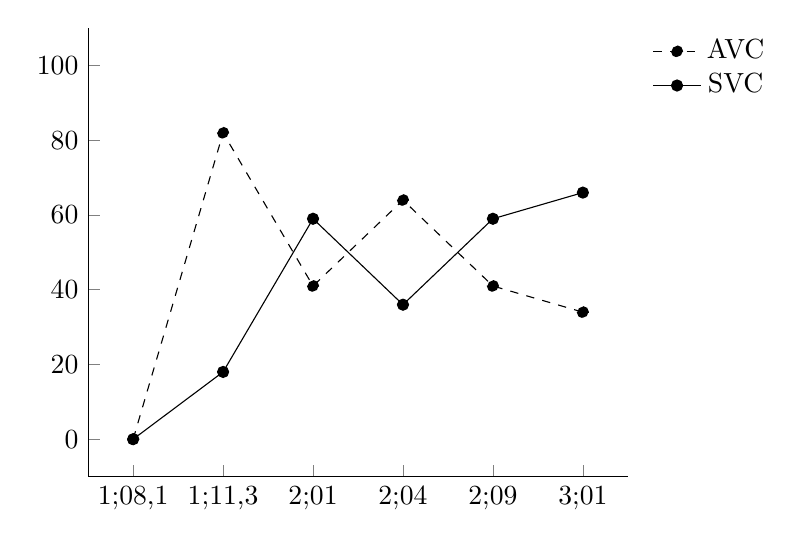
\begin{tikzpicture}
        \begin{axis}[
        	legend style={draw=none}, 
        	axis x line*=bottom,
            axis y line*=left,
            ymin = 0,
            ymax = 100,
            symbolic x coords = {{1;08,1}, {1;11,3}, 2;01, 2;04, 2;09, 3;01},
            enlargelimits =true,
			%x tick label style={rotate=90,anchor=east},
            legend pos = outer north east,
            xtick=data
          ]
            \addplot[dashed, color=black, mark=*] coordinates {
                ({1;08,1}, 0)
                ({1;11,3}, 82)
                (2;01, 41)
                (2;04, 64)
                (2;09, 41)
                (3;01, 34)
            };
            \addplot[color=black, mark=*] coordinates {
                ({1;08,1}, 0)
                ({1;11,3}, 18)
                (2;01, 59)
                (2;04, 36)
                (2;09, 59)
                (3;01, 66)
            };
            \legend{AVC,SVC}
        \end{axis}
    \end{tikzpicture}     
\end{figure}

\begin{figure}
 \caption{Relative incidence of AVC vs SVC types in the samples from \ili{Enita} (in \%)}
 \label{fig:rumsey:2}
 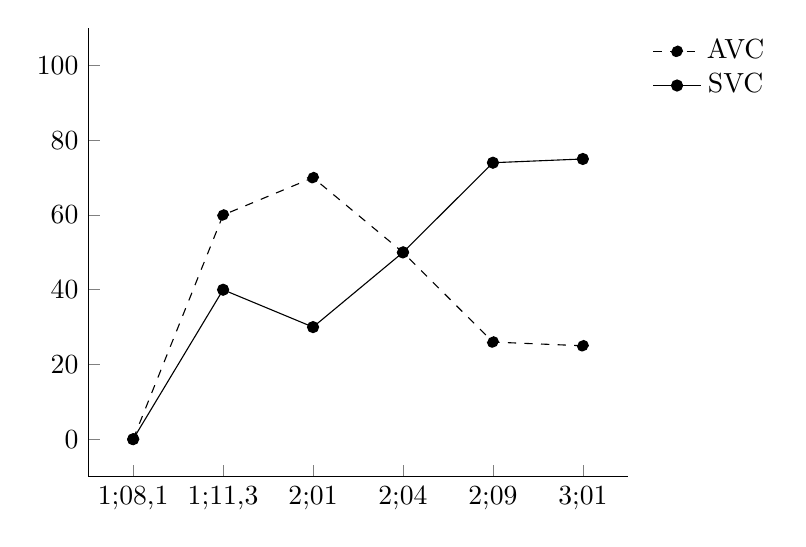
\begin{tikzpicture}
        \begin{axis}[
        	legend style={draw=none},
        	axis x line*=bottom,
            axis y line*=left,
            ymin = 0,
            ymax = 100,
            symbolic x coords = {{1;08,1}, {1;11,3}, 2;01, 2;04, 2;09, 3;01},
            enlargelimits =true,
			%x tick label style={rotate=90,anchor=east},
            legend pos = outer north east,
            xtick=data
          ]
            \addplot[dashed, color=black, mark=*] coordinates {
                ({1;08,1}, 0)
                ({1;11,3}, 60)
                (2;01, 70)
                (2;04, 50)
                (2;09, 26)
                (3;01, 25)
            };
            \addplot[color=black, mark=*] coordinates {
                ({1;08,1}, 0)
                ({1;11,3}, 40)
                (2;01, 30)
                (2;04, 50)
                (2;09, 74)
                (3;01, 75)
            };
            \legend{AVC,SVC}
        \end{axis}
    \end{tikzpicture}   
\end{figure}

\begin{figure}
 \caption{Relative incidence of AVC vs SVC tokens in the samples from Jesi (in \%)}
 \label{fig:rumsey:3}
 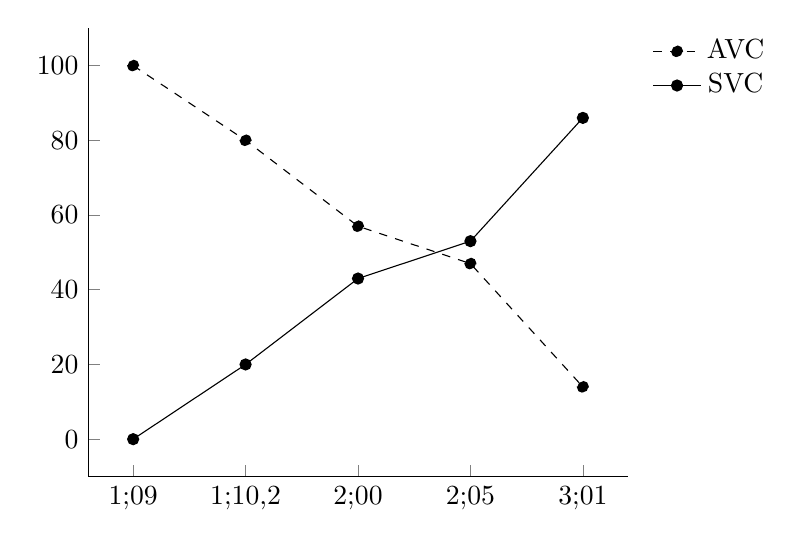
\begin{tikzpicture}
        \begin{axis}[
        	legend style={draw=none},
        	axis x line*=bottom,
            axis y line*=left,
            ymin = 0,
            ymax = 100,
            symbolic x coords = {1;09, {1;10,2}, 2;00, 2;05, 3;01 },
            enlargelimits =true,
			%x tick label style={rotate=90,anchor=east},
            legend pos = outer north east,
            xtick=data
          ]
            \addplot[dashed,mark=*,color=black] coordinates {
                (1;09,   100)
                ({1;10,2},  80)
                (2;00,   57)
                (2;05,  47)
                (3;01,  14)
            };
            \addplot[color=black,mark=*] coordinates {
                (1;09,   0)
                ({1;10,2},  20)
                (2;00,   43)
                (2;05,  53)
                (3;01,  86)
            };
            \legend{AVC,SVC}
        \end{axis}
    \end{tikzpicture}
\end{figure}

\begin{figure}
 \caption{Relative incidence of AVC vs SVC types in the samples from Jesi (in \%)}
 \label{fig:rumsey:4}
 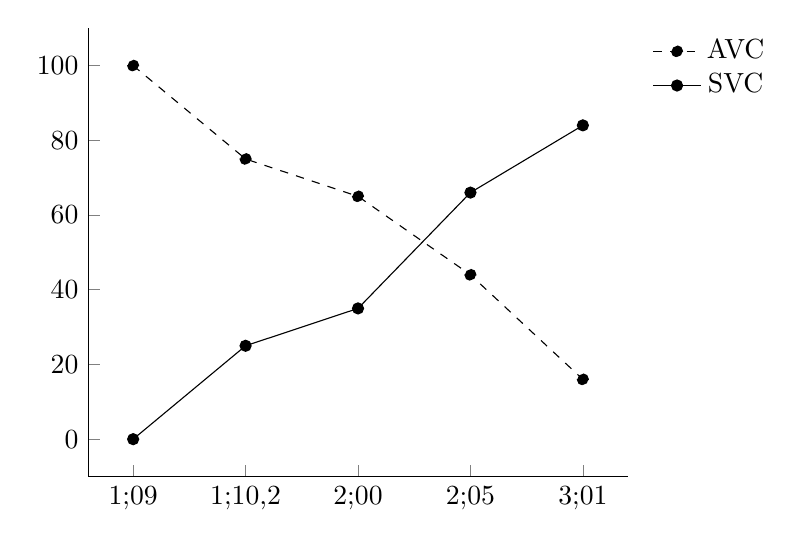
\begin{tikzpicture}
        \begin{axis}[
        	legend style={draw=none},
        	axis x line*=bottom,
            axis y line*=left,
            symbolic x coords = {1;09, {1;10,2}, 2;00, 2;05, 3;01 },
            enlargelimits =true,
			%x tick label style={rotate=90,anchor=east},
            legend pos = outer north east,
            xtick=data
          ]
            \addplot[dashed,mark=*,color=black] coordinates {
                (1;09,   100)
                ({1;10,2},  75)
                (2;00,   65)
                (2;05,  44)
                (3;01,  16)
            };
            \addplot[color=black,mark=*] coordinates {
                (1;09,   0)
                ({1;10,2},  25)
                (2;00,   35)
                (2;05,  66)
                (3;01,  84)
            };
            \legend{AVC,SVC}
        \end{axis}
    \end{tikzpicture} 
\end{figure}

\clearpage 

Besides verb constructions both children make regular use of verbless copular clauses of the kind exemplified from adult speech in (11), always with the subject NP in initial position and the predicate NP in final position, as in adult speech.  An example is (15).

\ea
    \glll i         na           popa        \\
    i        na-nga      pepa\\
        This    1\textsc{sg}-\textsc{gen}    paper\\
        \glt This is my paper. (Jesi, 2;00).
\z

Perhaps drawing on the model provided both by these verbless clauses and by AVCs such as (13a-b), children in the 20-25 month age range sometimes (albeit rarely) use adjuncts without accompanying verbs as full predications. An example is (16).

\ea
\glll      e      popa         \textbf{bi}\\
          ekepu   pepa-yl      \textbf{bi}      \textbf{ta-b}\\
          now    paper-\textsc{def}    write    hit:\textsc{opt}-1\textsc{sg}\\
          \glt `Now I'll write on the paper.' (Jesi, 2:00)
\z

\subsection{Discussion}

\is{children's speech} Comparing the above data from \ili{Ku Waru} children’s speech with adults’ we can see that in both, predicates always come last in the clause, and arguments come before them. In adult speech this means that the final element in the clause is almost always either a verb or, more rarely, a predicate nominal in a copular clause. The adjuncts in AVCs form part of the predicate, and always precede the inflected verb. In two-year olds' speech there is wider latitude, in that adjuncts are occasionally used in
final position as full predicates (as in 16). But in both adult speech and our samples from the two children, if there are one or more verbs in a clause, the final position is always occupied by one of them. Likewise, in both child language and adult speech, if the clause contains both an adjunct and an inflected verb, the verb always occurs after the adjunct and the two of them after any argument NP(s) that may occur in the clause.

\is{phrasal verb constructions} \is{serial verb constructions} A striking \textit{difference} between adults’ speech and the earliest samples from \ili{Enita} and Jesi is in the relative frequency of SVCs \textit{vs} AVCs. In our samples of speech among adults SVCs are roughly three times as frequent as AVCs. By contrast, as can be seen from Figures 1-4, in the children's speech, AVCs greatly outnumber SVCs at first, then begin to be outnumbered by them at about 2;03, until something close to the adult ratio is reached by 3;01. Both this dissimilarity and the commonalities I pointed to above may be understood in terms of the two fundamental patterns that I have described in §2.1, namely: 1) a strict mapping of the functions predicate and argument \is{predicates} \is{arguments} onto the clause positions final and non-final respectively, and 2) an overall right-to-left mapping of the word classes Verb, Adjunct,\footnote{My treatment of ‘adjunct’ in this chapter as both a word class and a structural position within the AVC is somewhat of an oversimplification in that there are actually two classes of words that can occur in that position. One of them – to which most such words belong – consists of words that can \textit{only} occur only in that position. These we call Adjuncts, distinguishing the word class from the structural position by the use of upper case for it. The other such words can occur either in that position or as a nouns with related senses, e.g. \textit{el} ‘arrow’/`fight’, \textit{numan} ‘mind’/ ‘to like’. These we call ‘flexibles’, after \citet{Luuk2010}. In line with Luuk’s use of that term, we treat words of this class, and also Adjuncts, as having an intermediate status between nouns and verbs. This is consistent with my claim that the \ili{Ku Waru} clause shows an overall mapping of the word classes verb, Adjunct, and noun onto the positions final, penultimate and antepenultimate respectively, and renders that mapping more iconic, since the word classes that fill the intermediate position in it have a paradigmatically intermediate status between the preceding and following ones. For a fuller treatment of these issues and discussion of them in relation to much of the same data that is treated in this paper see \citet{MerlanForthcoming}.} and Noun onto the positions final, penultimate and antepenultimate respectively. 

These two templates account for the similarities between child speech and adult speech because they are consistently found in both, suggesting that they are one of the most fundamental aspects of \ili{Ku Waru} grammar. They also account for the differences between child and adult speech in that a sequence of (NP)-Adjunct-Verb comprises a more straightforward realization of both templates than does the sequence (NP)-Verb-Verb, in at least two respects. First, it fills the verb slot in the Noun-Adjunct-Verb template with a single verb, from among the same set of words that the children have begun to learn first as simple verbs, and fills the adjunct slot with a word of a different class, which is never used by adults in final position, and almost never by children.  Second, it fills the\is{predicates}\is{arguments} predicate slot in the argument(s)-predicate template with a single element, an adjunct+verb collocation that is easier to process as a single constituent of the clause than is any serial verb construction, since the words that occur in the adjunct slot are invariant in form and more regularly combined with a single, specific verb root (or small number of alternative ones) than are any of the verbs that enter into SVCs. Underlying the latter consideration is a kind of fractal congruence between the \ili{Ku Waru} clause and AVC as verb-final constructions. \is{serial verb constructions} \is{phrasal verb constructions} 

\subsection{The role of adult input}

In §2.3 I made some use of data from a sample of adults’ speech to other adults, in which the ratio of SVC to AVC tokens was roughly 3 to 1. As discussed there, I compared that ratio with the SVC-AVC ratios in the samples of children’s speech treated in this study, and found that those are much lower than that adult ratio at first. But as seen from Tables \ref{tab:rumsey:4} and \ref{tab:rumsey:5} and figures 1-4, the SVC-AVC ratios greatly increase by 3;01, at which point they exceed the adult ratio in one of the children’s speech and approach it in the other’s. As another comparator it is important to consider not only speech by adults to other adults, but also the speech that was used by the adults and older children in their interaction with the children under study at each session that is being considered.\footnote{In all of the samples considered here, the amount of speech by adults to the children under study is far greater than the amount by other children, and in some there is none of the latter at all.} For that comparison I have done a count of the relevant tokens and types in the adults’ speech to \ili{Enita} at each of the sessions represented in table \ref{tab:rumsey:4}. Space restrictions preclude my presenting those findings in full (for which see \citealt{MerlanForthcoming}). Here I will simply note that:

\is{baby talk register} \is{phrasal verb constructions} \is{serial verb constructions}
\begin{itemize}
\item the frequency of both AVC and SVC in the children’s speech is lower – at first much lower – than in that of the adults’ speech to the children;
\item in the speech of adults and older children when interacting with the children there is a far higher ratio of AVC to SVC than in the sample of speech by adults to other adults.
\end{itemize}

The second of these two patterns is surely an important factor in accounting for why children begin to use AVCs before SVCs and why they continue to use them at higher rates than in adult-to-adult speech well into their third year at least. For as a large body of research has shown, other things being equal, \is{acquisition} children’s acquisition of given language structures is strongly affected by the relative frequency with which they occur in the speech of adults who speak to them \citep{Lieven2010,Ambridge2011}. But what accounts for pattern 2 itself? I suggest that an important factor there is the adults’ intuitive feel for the structural templates I have described in §2.3, and the entailed difference between AVCs and SVCs, whereby a sequence of (NP)-adjunct-verb comprises a more straightforward realization of both templates than does the sequence (NP)-verb-verb. In other words, when speaking to young children the adults orient towards to the use of maximally perspicuous structures that will be easier for children to acquire. 

\section{Conclusions}

\is{typology} \is{comparative typology} \is{markedness} As is richly exemplified by many of the chapters in this volume and the publications cited in them, there has been much debate among linguists about the nature and viability of cross-linguistic typological comparison, and in particular about the use in it of concepts of markedness. In the heat of that debate I think we are sometimes in danger of throwing the baby out with the bathwater, in that, quite understandably, it tends to highlight theoretical differences among the protagonists rather the common ground among them. With that in mind, in this chapter I have focused on concrete examples that I think demonstrate the validity of basic tenets that inform markedness theory in all its variants, but are generally also accepted by its critics. One is the common-sense notion that some linguistic phenomena are simpler than others, and partly for that reason easier for children to learn, and are therefore learned at a younger age. This is exemplified in §1 by \ili{Ku Waru} children’s much earlier production of the apico-alveolar lateral /l/ than the pre-stopped velar lateral /{\gL}/, and in §2 by their earlier production of simple verbs than of complex verb constructions. I take it that nearly all linguists, regardless of their differences in other respects, would agree with my judgments as to relative simplicity \textit{vs} complexity in these two cases, and with my claim that those differences can be related to the differences in order of acquisition. The relation between those two kinds of difference is one of what I would call ``relative determination", in that the greater simplicity of /l/ and of `simple verbs" at least in part determines the order of their acquisition. \is{acquisition} 

\is{universals} \is{simplicity vs. complexity} \is{baby talk register} The kinds of simplicity involved in the above examples are, I would claim, universal, or intrinsic to the phenomena themselves. That is, [l] is inherently simpler in its manner of articulation than [{{\gL}}]  and a single verb is inherently simpler than a construction that includes it. In addition to these examples of intrinsic simplicity, I have also discussed kinds of simplicity \textit{vs} complexity that are relational and language-specific. On the phonological side, these included the placement of [{{\gL}}]  as a (pre-stopped) lateral rather than a (laterally released) stop, which I argued is a determining factor in its baby-talk pronunciation as [l]. On the syntactic side, I argued that \ili{Ku Waru} children’s earlier acquisition of AVCs than SVCs was determined in part by the greater structural congruence between AVCs with basic aspects of the structure of the \ili{Ku Waru} clause. Note that in both of these cases, while the phenomena in question are language specific, my accounts of them appeal to what are widely agreed to be universal tendencies in language: a tendency towards pattern congruity \is{pattern congruity} \is{structural congruity} in phonology and a tendency in syntax toward structural congruence, or what \citet{greenberg1966universals} called ``harmony" among construction types within a given language.  While my arguments about these particular \ili{Ku Waru} phenomena may be disputed, the universal tendencies on which they are based seem to me by now very well established,\footnote{For phonological examples see Hyman, this volume, Rice, this volume, and references therein. For rich comparative data supporting many of Greenberg’s generalizations regarding word order see \citet{Dryer1992greenbergian,Hawkins2014}.} as does the determining role they play in children’s language acquisition.  As can be seen from both examples treated here, the influence of such patterning is shown not only in the way children simplify the language when speaking it, but also in the way that adults simplify it when speaking to them, in effect manifesting what I have called an ``intuitive feel" for the operation of markedness hierarchies within their language.

\section*{Acknowledgements}

For their helpful comments on earlier versions of this chapter I thank Katherine Demuth, Francesca Merlan, Hannah Sarvasy, and Tony Woodbury. For their advice concerning aspects of the discussion in §1 thanks to Alex François and Ian Maddieson. For funding the research on which the chapter is based I gratefully acknowledge the \ili{Australian} Research Council and the \ili{Australian} National University.


\section*{Abbreviations not included in the Leipzig Glossing Rules}
\begin{tabular}{ll}
\textsc{idf} &  indefinite       \\
\textsc{nf} &  non-final\\
\end{tabular}
\begin{tabular}{ll}
\textsc{ppr} & present progressive\\   
\textsc{rp}  & remote past\\           
\end{tabular}


{\sloppy
\printbibliography[heading=subbibliography,notkeyword=this]
}

\end{document}
